% This example requires PGF >= 1.09 and only works wit PDFTeX
% You have to compile document twice to get correct placement of nodes.
\documentclass{standalone} %
\usepackage{tikz}
\usepackage{verbatim}

\usetikzlibrary{arrows,shapes,backgrounds}

\newcommand{\comparison}[4]{
#2 & \includegraphics[width=1cm]{#1.png} \raisebox{.5cm}{\tikz[na]\coordinate (s-#1);} & & \raisebox{.5cm}{\tikz[na]\coordinate (t-#3);} \includegraphics[width=1cm]{#3.png} & #4\\
}

\begin{document}
\tikzstyle{every picture}+=[remember picture]
\tikzstyle{na} = [baseline=-.5ex]
 
\begin{tabular}{rlp{6cm}lr}
\comparison{81}{16137}{17}{2438}
\comparison{25}{7081}{76}{729}
\comparison{76}{3798}{91}{554}
\comparison{46}{2981}{89}{527}
\comparison{22}{2546}{46}{506}
\comparison{48}{2332}{75}{275}
\comparison{89}{2197}{88}{269}
\comparison{91}{2066}{22}{245}
\comparison{94}{1795}{48}{222}
\comparison{101}{1717}{25}{208}
\comparison{75}{1431}{49}{186}
\comparison{88}{1397}{50}{185}
\comparison{19}{1291}{16}{185}
\comparison{53}{1216}{18}{180}
\comparison{66}{1192}{67}{168}
\comparison{108}{1125}{94}{167}
\comparison{82}{1057}{81}{155}
\comparison{49}{941}{66}{150}
\comparison{20}{933}{73}{143}
\comparison{52}{889}{97}{140}
\comparison{97}{836}{53}{137}
\comparison{17}{763}{51}{135}
\comparison{51}{729}{52}{103}
\comparison{50}{712}{20}{92}
\comparison{67}{651}{82}{85}
\comparison{16}{605}{19}{72}
\comparison{73}{568}{101}{69}
\comparison{18}{501}{108}{7}

% \includegraphics[width=2cm]{88.png} \tikz[na]\coordinate (s-88); & 12 & 17 & \ \tikz[na]\coordinate (t-76); 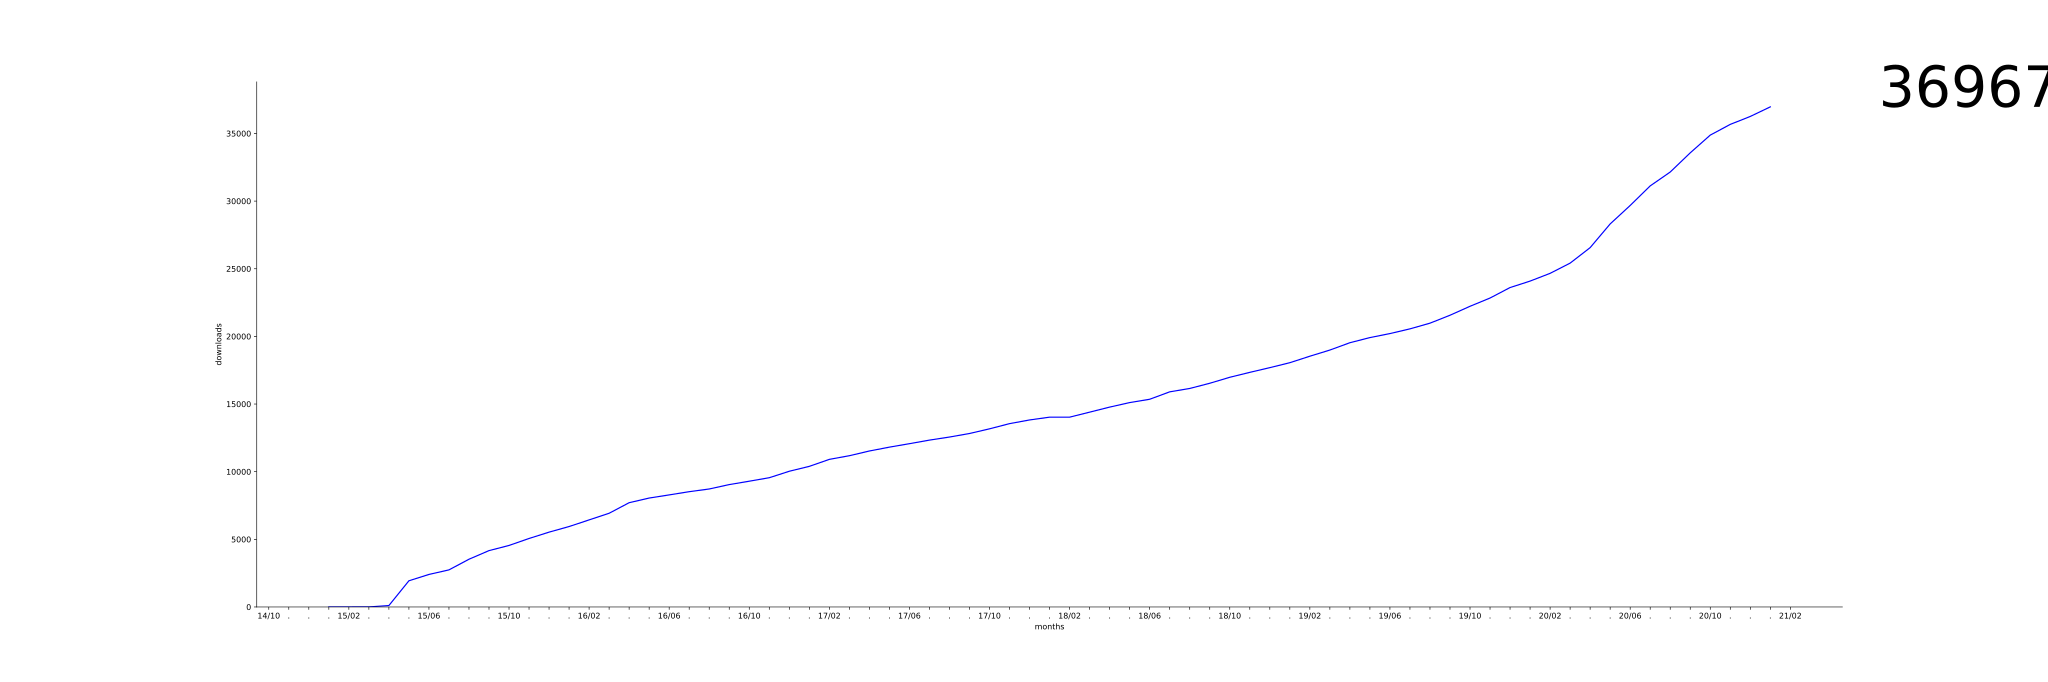
\includegraphics[width=2cm]{76.png}\\
% 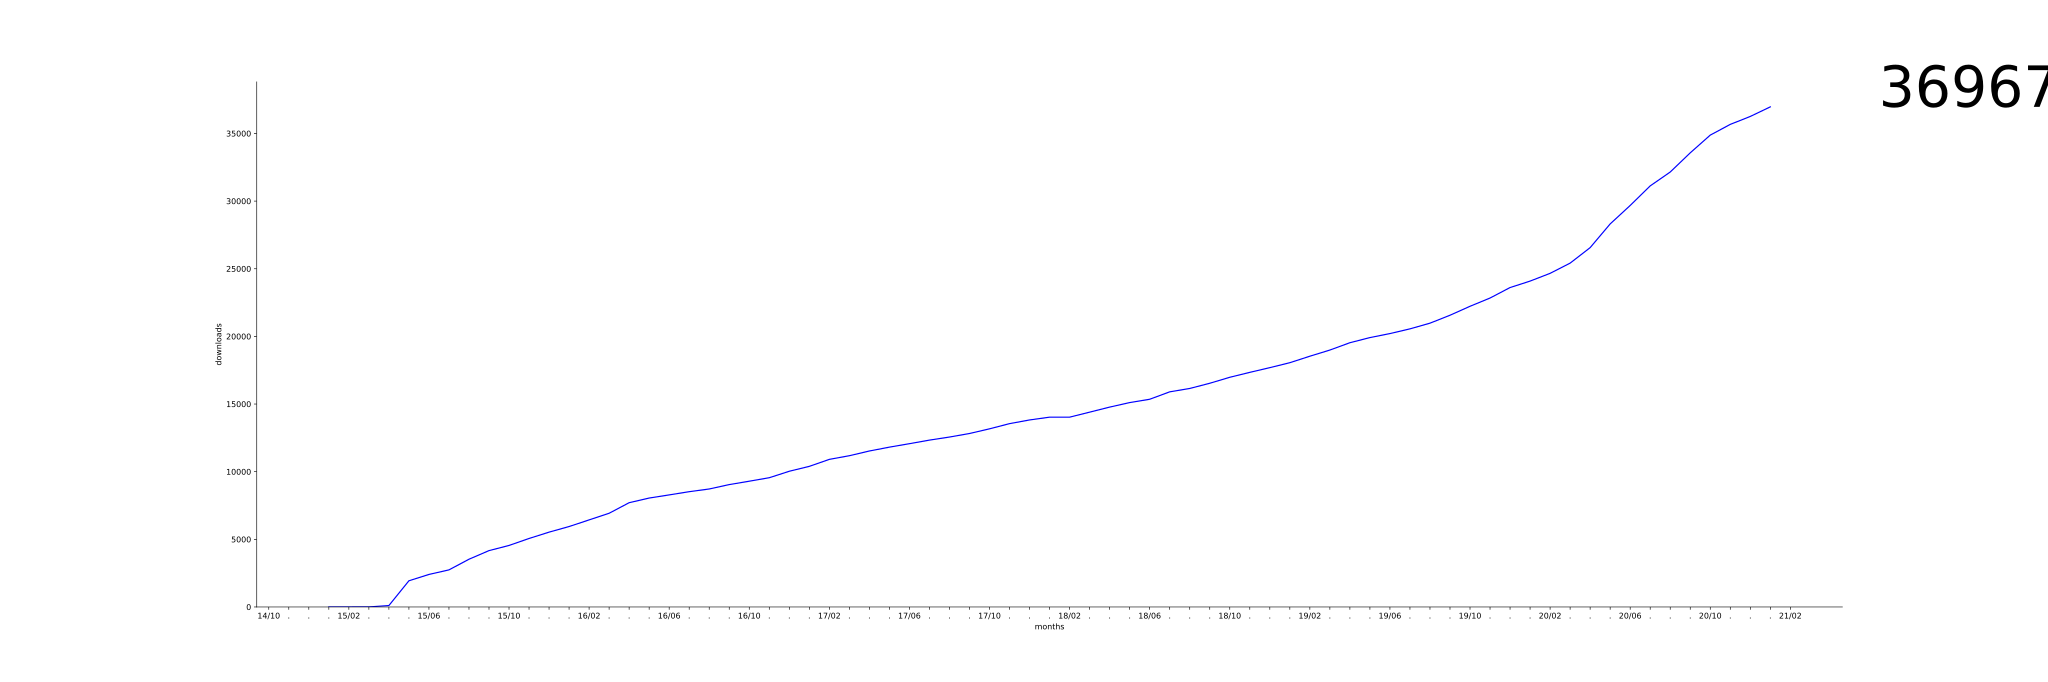
\includegraphics[width=2cm]{76.png} \tikz[na]\coordinate (s-76); & 11 & 13 &  \tikz[na]\coordinate (t-88); \includegraphics[width=2cm]{88.png}\\
\end{tabular}

\newcommand{\connect}[2]{ \path[-,#2,thick] (s-#1) edge  (t-#1);}
\begin{tikzpicture}[overlay]
\connect{81}{red}
\connect{25}{blue}
\connect{76}{green}
\connect{46}{orange}
\connect{22}{gray}
\connect{48}{brown}
\connect{89}{purple}
\connect{91}{black}
\connect{94}{pink}
\connect{75}{red}
\connect{88}{blue}
\connect{19}{green}
\connect{53}{orange}
\connect{66}{gray}
\connect{82}{brown}
\connect{49}{purple}
\connect{20}{black}
\connect{52}{pink}
\connect{97}{red}
\connect{17}{blue}
\connect{51}{green}
\connect{50}{orange}
\connect{67}{gray}
\connect{16}{brown}
\connect{73}{purple}
\connect{18}{black}
\connect{101}{pink}
\connect{108}{red}
\end{tikzpicture}
 

\end{document}